\chapter{Preliminaries}
\label{ch:prelim}
This chapter provides a mathematical background for understanding 
Galois fields and explains how to design Galois field arithmetic circuits.
Specifically, this chapter covers monomial ordering, polynomial ideals and 
varieties, and the computation of \Grobner bases.
Moreover, we introduce the mathematical concepts of groups, rings, fields, and 
polynomials. 
We then apply these concepts to create Galois field arithmetic functions and 
explain how elimination and abstraction on Galois field works.
The material is referred from \cite{galois_field:mceliece} \cite{ftheory:2006} \cite{ff:1997} for Galois field concepts,
\cite{ideals:book} \cite{gb_book} for commutative algebra basics and 
previous work by {\it Lv} \cite{lv:phd} and {\it Pruss} \cite{tim:phd}.

\section{Commutative Algebra}
\label{sec:algebra}
\subsection{Group, ring and field}
\begin{Definition}
An {\bf abelian group} is a set $\mathbb{S}$ with a binary operation $'+'$
which satisfies the following properties: 
\begin{itemize}
\item {\it Closure Law:} For every $a, b \in \mathbb{S}, a + b \in \mathbb{S}$  
\item {\it Associative Law:} For every $a, b, c \in \mathbb{S}, (a + b) + c = a + (b + c)$
\item {\it Commutativity:} For every $a, b \in \mathbb{S}, a + b = b + a$. 
\item {\it Additive Identity:} There is an identity element $0 \in \mathbb{S}$
such that for all $a \in \mathbb{S};$ $a + 0 = a$.
\item {\it Additive Inverse:} If $a \in \mathbb{S}$, then there is an
element $a^{-1} \in \mathbb{S}$ such that $ a + a^{-1} = 0$.
\end{itemize}
\end{Definition}

The set of integers $\mathbb{Z}$ forms an abelian group under the addition operation. 

\begin{Definition}
Given a set $\mathbb{R}$ with two binary operations, $'+'$ and $'\cdot'$, 
and element $0 \in \mathbb{R}$, the system $\mathbb{R}$ is called a {\bf commutative ring with unity} if the following properties hold:
\begin{itemize}
\item $\mathbb{R}$ forms an abelian group under the '+' operation with additive identity element $0$.
\item {\it Multiplicative Distributive Law}: For all $a, b, c \in$ $\mathbb{R}$, $a\cdot (b + c) = a\cdot b + a\cdot c$.
\item {\it Multiplicative Associative Law}: For every $a, b, c\in \mathbb{R}$, $a\cdot (b\cdot c) = (a\cdot b)\cdot c$. 
\item {\it Multiplicative Commutative Law}: For every $a,b \in \mathbb{R}$, $a\cdot b = b\cdot a$
\item {\it Identity Element}: There exists an element $1 \in$ $\mathbb{R}$ 
such that for all $a \in \mathbb{R}$, $a\cdot 1 = a =1\cdot a$
\end{itemize}
\end{Definition}

For the purpose of this dissertation, any time we refer to a {\bf ring}, we are 
specifically referring to a {\bf commutative ring with unity}. Two common 
examples of such rings are the set of integers, $\mathbb{Z}$, and the set of 
rational numbers, $\mathbb{Q}$. Note that while both of these examples are
rings with an infinite number of elements, the number of elements in a ring 
can also be finite.

\begin{Definition}
A {\bf field} $\mathbb{F}$ is a commutative ring with unity, where every
non-zero element in $\mathbb{F}$ has a multiplicative inverse; i.e. $\forall
a \in \mathbb{F} - \{0\}$, $\exists \hat{a} \in \mathbb{F}$ such that $ a \cdot
\hat{a} = 1$.
\end{Definition}

A field is defined as a ring with one extra condition: the presence of a 
multiplicative inverse for all non-zero elements.
Therefore, a field must be a ring while a ring is not necessarily a field.
For example, the set $\mathbb{Z}_{2^k} = \{0,1,\cdots, 2^k-1\}$ forms a finite ring.
However, $\mathbb{Z}_{2^k}$ is not a field because not every element in
$\mathbb{Z}_{2^k}$ has a multiplicative inverse. 
In the ring $\mathbb{Z}_{2^3}$, for 
instance, the element $5$ has an inverse ($5\cdot5\pmod{8}=1$) but the element $4$
does not.

The main concept of field theory is {\bf Field Extensions}. The idea behind a
field extension is to take a base field and construct a larger field which 
contains the base field as well as satisfies additional properties. For example,
the set of real numbers $\mathbb{R}$ forms a field; one common extension of 
$\mathbb{R}$ is the set of complex numbers $\mathbb{C}=\mathbb{R}(i)$. Every
element of $\mathbb{C}$ can be represented as $a+b\cdot i$ where $a,b \in \mathbb{R}$,
hence $\mathbb{C}$ is a two-dimensional extension of $\mathbb{R}$.

Like rings, fields can also contain either an infinite or a finite number of 
elements. 
In this dissertation we focus on finite fields, also known as Galois fields, and 
the construction of their field extensions.

\subsection{Galois Field}
Galois fields, also known as finite fields, find widespread applications in 
many areas of electrical engineering and computer science such as error-
correcting codes, elliptic curve cryptography, digital signal processing, 
testing of VLSI circuits, among others.
In this dissertation, we specifically focus on their application to 
Elliptic Curve Cryptography as Galois field arithmetic circuits.
This section describes the relevant Galois field concepts
\cite{galois_field:mceliece} \cite{ftheory:2006} \cite{ff:1997}
and hardware arithmetic designs over such fields \cite{mastro:1989} \cite{PT:1985} 
\cite{acar:1998} \cite{wu:2002} \cite{Knezevic:2008}. 

%%%%%%%%%%%%%%%%%%%%%%%%%%%%%%%%%%%%%%%%%%%%%%%%%%%%%%%%%%%%%%%%%%%%%%%%%%%%

\begin{Definition} 
A {\bf Galois field}, denote $\Fq$, is a field with a finite
number of elements, $q$. The number of elements $q$ of the Galois field is
a power of a prime integer, i.e. $q = p^k$, where $p$ is a prime
integer, and $k \geq 1$. Thus a Galois field can also be denoted as 
$\F_{p^{k}}$.
\end{Definition}

Fields in the form $\F_{p^{k}}$ are called Galois extension fields.
We are specifically interested in extension fields of type 
$\Fkk$, where $k > 1$. These are extensions of the binary
field $\F_2$.
\begin{Example}
Addition and multiplication operations over $\F_2$:
\begin{table}[!h]
	\centering
	\begin{tabular}{m{1cm}|l|ll|m{1cm}}
	\hhline{~---~}
	\multirow{3}{*}{} & $+$ & $0$ & $1$ & \multirow{3}{*}{} \\
	\hhline{~---~}
	& $0$ & $0$ & $1$ & \\
	& $1$ & $1$ & $0$ & \\
	\hhline{~---~}
	\multicolumn{5}{c}{}\\
	\multicolumn{5}{c}{Addition over $\F_2$}\\
	\end{tabular}
	\quad
	\begin{tabular}{m{1cm}|l|ll|m{1cm}}
	\hhline{~---~}
	\multirow{3}{*}{} & $\cdot$ & $0$ & $1$ & \multirow{3}{*}{} \\
	\hhline{~---~}
	& $0$ & $0$ & $0$ & \\
	& $1$ & $0$ & $1$ & \\
	\hhline{~---~}
	\multicolumn{5}{c}{}\\
	\multicolumn{5}{c}{Multiplication over $\F_2$}\\
	\end{tabular}
\end{table}

Notice that addition over $\F_2$ is a Boolean {\sc XOR} operation, 
because it is performed modulo $2$.
Similarly, multiplication over $\F_2$ performs a Boolean {\sc AND} operation.
\end{Example}

Algebraic extensions of the binary field $\F_{2}$  
are generally termed as {\it binary extension fields} $\Fkk$.
Where elements in $\F_2$ can only represent $1$ bit, elements in $\Fkk$ 
represent a $k$-bit vector.
This allows them to be widely used in digital hardware applications.
In order to construct a Galois field of the form $\Fkk$, 
an {\bf irreducible polynomial} is required:
\begin{Definition}
A polynomial $P(x) \in \mathbb{F}_{2}\left[x\right]$ is {\bf irreducible} 
if $P(x)$ is non-constant with degree $k$ and cannot be 
factored into a product of polynomials of lower degree in $\mathbb{F}_2[x]$.
\end{Definition}

Therefore, the polynomial $P(x)$ with degree $k$ is irreducible over 
$\mathbb{F}_{2}$ if and only if it has no roots in $\mathbb{F}_{2}$,
i.e if $\forall a \in \mathbb{F}_{2}$, $P(a)\neq 0$.
For example, $x^2+x+1$ is an irreducible polynomial over $\mathbb{F}_{2}$
because it has no solutions in $\mathbb{F}_{2}$, i.e. $(0)^2+(0)+1=1\neq0$ 
and $(1)^2+(1)+1=1\neq0$ over $\F_2$.
Irreducible polynomials exist for any degree $\geq 2$ in $\mathbb{F}_2[x]$.

Given an irreducible polynomial $P(x)$ of degree $k$ in the polynomial ring 
$\mathbb{F}_2[x]$, we can construct a binary extension field 
$\mathbb{F}_{2^k} \equiv \mathbb{F}_2[x] \pmod{P(x)}$.
Let $\alpha$ be a root of $P(x)$, i.e., $P(\alpha)=0$.
Since $P(x)$ is irreducible over
$\mathbb{F}_2[x]$, $\alpha \notin \mathbb{F}_2$. 
Instead, $\alpha$ is an element in $\mathbb{F}_{2^k}$. 
Any element $A \in \mathbb{F}_{2^k}$ is then represented as: 
\begin{equation}\label{rep:poly}
A= \sum_{i=0}^{k-1} (a_i \cdot \alpha^i) = a_0 + a_1\cdot\alpha + \cdots + a_{k-1}\cdot \alpha^{k-1}\nonumber
\end{equation}
where $a_i \in \mathbb{F}_2$ are the coefficients and $P(\alpha)=0$.

To better understand this field extension, compare its similarities to another
common-place
field extension $\C$, the set of complex numbers. $\C$ is an extension of the field 
of real numbers $\R$ with an additional element $i=\sqrt{-1}$, which is an imaginary
root in $\R$.
Thus $i \notin \R$, rather $i \in \C$.
Every element $A \in \mathbb{C}$ can be represented as:
\begin{equation}\label{rep:polyC}
A=\sum_{j=0}^{1} (a_j \cdot i^j)=a_0+a_1\cdot i
\end{equation}
where $a_j \in \R$ are coefficients. Similarly, $\Fkk$ is an extension of $\F_2$ with 
an additional element $\alpha$, which is the ``imaginary root'' of an irreducible 
polynomial $P$ in $\F_2[x]$.

Every element $A \in \Fkk$ has a degree less than $k$ because 
$A$ is always computed modulo $P(x)$, which has degree $k$. 
Thus, $A\pmod {P(x)}$ can be of degree at most $k-1$ and at least $0$.
For this reason, the field $\mathbb{F}_{2^k}$ can be viewed as a $k$
dimensional vector space over $\mathbb{F}_{2}$. 
The equivalent bit vector representation for element $A$ is:
\begin{equation}
A=(a_{k-1} a_{k-2} \cdots a_{0})
\end{equation}

\begin{Example}
A 4-bit Boolean vector, $(a_{3} a_{2} a_{1} a_{0})$
can be presented over $\F_{2^4}$ as: 
\begin{equation}
a_3 \cdot \alpha^3+a_2 \cdot \alpha^2+a_1 \cdot \alpha+a_0
\end{equation}
For instance, the Boolean vector $1011$ is represented as the element 
$\alpha^3+\alpha+1$.
\end{Example}

\begin{Example}\label{exp:1}
Let us construct $\mathbb{F}_{2^4}$ as $\mathbb{F}_2[x] \pmod{ P(x)}$, where
$P(x)=x^4+x^3+1 \in \mathbb{F}_2[x]$ is an irreducible polynomial of degree $k=4$. 
Let $\alpha$ be the root of $P(x)$, i.e. $P(\alpha)=0$. 

Any element $A \in \mathbb{F}_2[x] \pmod{ x^4 + x^3 + 1}$
has a representation of the type: $A = a_3 x^3 + a_2 x^2 +
a_1 x + a_0$ (degree $< 4$) where the coefficients $a_3, \dots, a_0$ are in $\F_2 =
\{0, 1\}$. Since there are only $16$ such polynomials, we obtain
$16$ elements in the field $\mathbb{F}_{2^4}$. Each element in
$\mathbb{F}_{2^4}$ can then be viewed as a $4$-bit vector over $\mathbb{F}_{2}$. 
Each element also has an exponential $\alpha$
representation. All three representations are shown in Table
\ref{tab:gfelement}.

\begin{table}[h]
\begin{center}
\caption{Bit-vector, Exponential and Polynomial representation of
elements in  $\mathbb{F}_{2^4} = \mathbb{F}_2[x] \pmod{x^4+x^3+1}$}\label{tab:gfelement} 
\begin{tabular}{|c|c|c||c|c|c|} 
\hline
$a_3a_2a_1a_0$ & Exponential & Polynomial     &$a_3a_2a_1a_0$ & Exponential & Polynomial  \\
\hline
$0000$        & $0$         & $0$            & $1000$ & $\alpha^3$ &  $\alpha^3$\\
\hline
$0001$        & $1$         & $1$            & $1001$ & $\alpha^4$ & $\alpha^3 + 1$\\
\hline
$0010$        & $\alpha$    & $\alpha$       & $1010$ & $\alpha^{10}$&$\alpha^3 + \alpha$  \\
\hline
$0011$        & $\alpha^{12}$& $\alpha + 1$   & $1011$ & $\alpha^5$ & $\alpha^3+\alpha+1$\\
\hline
$0100$        & $\alpha^2$  & $\alpha^2$     &  $1100$ & $\alpha^{14}$ & $\alpha^3 + \alpha^2$\\
\hline
$0101$        & $\alpha^9$   &$\alpha^2 + 1$ & $1101$  &$\alpha^{11}$  & $\alpha^3+\alpha^2+1$\\
\hline
$0110$        & $\alpha^{13}$& $\alpha^2 + \alpha$ & $1110$ & $\alpha^8$& $\alpha^3+\alpha^2+\alpha$\\
\hline
$0111$        &$\alpha^7 $ & $\alpha^2+\alpha+1$ & $1111$ &$\alpha^6$ & $\alpha^3+\alpha^2+\alpha+1$\\
\hline
\end{tabular}
\end{center}
\end{table}

We can compute the polynomial representation from the exponential representation.
Since every element is computed $\pmod{P(\alpha)} = \pmod{\alpha^4+\alpha^3+1}$, 
we compute the element $\alpha^{4}$ as 
\begin{equation}
\alpha^{4} \pmod{ \alpha^4+\alpha^3+1} = -\alpha^3 - 1 = \alpha^3+1
\end{equation}
Recall that all coefficients of $\F_{2^4}$ 
are in $\F_{2}$ where $-1 = +1$ modulo 2.
The next element $\alpha^{5}$ can be computed as 
\begin{equation}
\alpha^{5} = \alpha^{4}\cdot \alpha = (\alpha^3+1)\cdot \alpha = \alpha^4+\alpha = \alpha^3+\alpha+1 
\end{equation}
Then $\alpha^6$ can be computed as $\alpha^{5}*\alpha$ and so on.
\end{Example}

An irreducible polynomial can also be a primitive polynomial.

\begin{Definition}
A {\bf primitive polynomial} $P(x)$ is a polynomial with coefficients in $\mathbb{F}_2$ 
which has a root $\alpha$ $\in$ $\mathbb{F}_{2^k}$
such that \{$0$, $1(=\alpha^{{2^k}-1})$, $\alpha$, $\alpha^2$, $\cdots$, $\alpha^{2^k-2}$\} is the set of 
all elements in $\mathbb{F}_{2^k}$, 
where $\alpha$ is a {\bf primitive element} of $\mathbb{F}_{2^k}$. 
\end{Definition}

A primitive polynomial is guaranteed to generate all distinct elements 
of a finite field $\mathbb{F}_{2^k}$ while an irreducible polynomial
has no such guarantee.
Often, there exists more than one irreducible polynomial of degree $k$.
In such cases, any degree $k$ irreducible polynomial can be 
used for field construction. For example, both $x^3+x+1$ and $x^3+x^2+1$ 
are irreducible in $\mathbb{F}_2$ and either one can be used
to construct $\mathbb{F}_{2^3}$. This is due to the following:

\begin{Theorem}\label{the:unique}
There exist a {\bf unique} field $\mathbb{F}_{p^k}$, for any prime $p$ and any positive integer $k$.
\end{Theorem}

Theorem \ref{the:unique} implies that Galois fields with the same number of elements are 
{\bf isomorphic} to each other up to the labeling of the elements. 

Theorem \ref{the:fer} provides an important property for investigating solutions to
polynomial equations in $\Fq$.

\begin{Theorem}\label{the:fer}
 $\left[Generalized\  Fermat's\  Little\  Theorem \right]$ Given a
 Galois field $\mathbb{F}_{q}$, each element $A \in \mathbb{F}_{q}$ satisfies: 
\begin{eqnarray}\label{fe}
 A^{q} & \equiv & A  \nonumber \\
 A^{q} - A & \equiv& 0  
\end{eqnarray}
\end{Theorem} 

We can extend Theorem \ref{the:fer} to polynomials in $\mathbb{F}_{q}[x]$ as 
follows: 
\begin{Definition}
Let $x^q-x$ be a polynomial in $\mathbb{F}_{q}[x]$.
Every element $A \in \mathbb{F}_{q}$ is a solution to  $x^q-x=0$. 
Therefore, $x^{q} - x$ always {\it vanishes} in $\mathbb{F}_{q}$. Such 
polynomials are called {\bf vanishing polynomials} of the field $\mathbb{F}_{q}$.
\end{Definition}

\begin{Example}
Given $\mathbb{F}_{2^2} =\{0,1,\alpha,\alpha+1\}$ with $P(x)=x^2+x+1$, where $P(\alpha)=0$. 
 \begin{eqnarray}
 0^{2^2}&=&0 \nonumber \\
 1^{2^2}&=&1 \nonumber \\
 \alpha^{2^2}&=&\alpha \pmod {\alpha^2+\alpha+1}\nonumber \\
 (\alpha+1)^{2^2}&=&\alpha+1 \pmod {\alpha^2+\alpha+1} \nonumber 
 \end{eqnarray}
\end{Example}

A Galois field $\F_q$ can be fully contained within a larger field $\F_{q^k}$.
That is, $\F_q \subset \F_{q^k}$.
For example, Fig \ref{fig:contain2_4_16} shows the containment of the fields 
$\F_2 \subset \F_4 \subset \F_{16}$. It's easy to see that since $\F_4=\F_{2^2}$, it
contains $\F_2$. Likewise $\F_{16}=\F_{4^2}=\F_{2^4}$ contains $\F_4$ and $\F_2$.
The elements $\{0,1,\alpha,\dots,\alpha^{14}\}$
designate $\F_{16}$. Of these, $\{0,1,\alpha^5,\alpha^{10}\}$ create $\F_4$.
From these, only $\{0,1\}$ exist in $\F_2$.

\begin{Theorem}
$\F_{2^n}\subset\F_{2^m}$ iff $n \mid m$, i.e. if $n$ divides $m$.
\end{Theorem}

Therefore:
\begin{itemize}
\item $\F_2 \subset \F_{2^2} \subset \F_{2^4} \subset \F_{2^8} \subset \dots$
\item $\F_2 \subset \F_{2^3} \subset \F_{2^9} \subset \F_{2^{27}} \subset \dots$
\item $\F_2 \subset \F_{2^5} \subset \F_{2^{25}} \subset \F_{2^{125}} \subset \dots,$ and so on
\end{itemize}

\begin{Definition}
The {\bf algebraic closure} of the Galois field $\F_{2^k}$, denoted $\overline{\Fkk}$, is the 
union of all fields $\F_{2^n}$ such that $k \mid n$.
\end{Definition}

% TODO \Fkk operations example

\subsection{Monomials, Polynomials and Polynomial Arithmetics}
\begin{Definition} \label{def:mono}
A {\bf monomial} in variables $x_1,x_2,\cdots,x_d$ is a product of the form:
\begin{equation}
x_1^{{\alpha}_1} \cdot x_2^{{\alpha}_2} \cdot \cdots x_d^{{\alpha}_d},
\end{equation}
where $\alpha_i \ge 0, i\in\{1,\cdots,d\}$. 
The total degree of the monomial is $\alpha_{1}+\cdots+\alpha_{d}$.
\end{Definition} 

Thus, $x^2\cdot y$ is a monomial in variables $x,y$ with total degree $3$.
For simplicity, we will henceforth denote a 
monomial $x_1^{{\alpha}_1} \cdot x_2^
{{\alpha}_2} \cdot \cdots x_d^{{\alpha}_d}$ as $x^{\alpha}$, 
where $\alpha=({\alpha}_1,\cdots,{\alpha}_d)$ is a vector size $d$ of 
integers $\ge 0$, i.e., $\alpha \in \mathbb{Z}_{\ge 0}^{d}$.

\begin{Definition}\label{def:poly}
Let $\mathbb{R}$ be a ring. A {\bf polynomial} over $\mathbb{R}$ in the 
indeterminate $x$ is an expression of the form:
\begin{equation} \label{eq:poly1}
a_0 + a_1 x + a_2 x^2 + \cdots + a_k x^k = \sum_{i=0}^{k} a_i x^i, \forall a_i \in \mathbb{R}. 
\end{equation}

\end{Definition}

The constants $a_i$ are the coefficients and $k$ is the degree of the polynomial. 
For example, $8x^3 + 6x + 1$ is a polynomial in $x$ over $\mathbb{Z}$, with
coefficients $8$, $6$, and $1$ and degree $3$. 

\begin{Definition}
The set of all polynomials in the indeterminate
$x$ with coefficients in the ring $\mathbb{R}$ forms a {\bf
ring of polynomials} $\mathbb{R}[x]$. 
Similarly, $\mathbb{R}[x_1,x_{2},\cdots, x_{n}]$ 
represents the ring of multivariate polynomials with coefficients in $\mathbb{R}$.
\end{Definition}

For example, $\mathbb{Z}_{2^4}[x]$ stands for the set of all polynomials in
$x$ with coefficients in $\mathbb{Z}_{2^4}$. $8x^3 + 6x + 1$ is an instance 
of a polynomial contained in $\mathbb{Z}_{2^4}[x]$.

\begin{Definition}
A {\bf multivariate polynomial} $f$ in variables $x_1, x_2, \ldots, x_d$ 
with coefficients in any given field $\K$ is a finite linear 
combination of monomials with coefficients in $\K$: 
\begin{equation}
	f=\sum_{\alpha}a_{\alpha}\cdot x^{\alpha}, ~~a_{\alpha}\in \K \nonumber
\end{equation}

The set of all polynomials in $x_1, x_2, \ldots, x_d$ with coefficients in 
field $\K$ is denoted by $\K[x_1, x_2, \ldots, x_d]$. 
Thus, $f \in \K[x_1, x_2, \ldots, x_d]$

\begin{enumerate}
\item We refer to the constant $a_{\alpha} \in \K$ as the 
{\bf coefficient} of the monomial $a_{\alpha} x^{\alpha}$.
\item If $a_{\alpha} \neq 0$, we call $a_{\alpha} x^{\alpha}$ a term of $f$.
\end{enumerate}
\end{Definition}

As an example, $2x^2+y$ is a polynomial with two terms $2x^2$ and $y$, with 
$2$ and $1$ as coefficients respectively. 
In contrast, $x+y^{-1}$ is not a polynomial because the exponent of $y$ is 
less than $0$.

Since a polynomial is a sum of its terms,
these terms have to be arranged unambiguously so that they can be 
manipulated in a consistent manner.
Therefore, we need to establish a concept of 
{\bf term ordering} (also called monomial ordering).
A term ordering, represented by $>$, defines how
terms in a polynomial are ordered.

Common term orderings are lexicographic ordering (LEX) and its variants: 
degree-lexicographic ordering (DEGLEX) and reverse degree-lexicographic ordering (DEGREVLEX).

A {\bf lexicographic ordering} (lex) is a total-ordering $>$ such that 
variables in the terms are lexicographically ordered, i.e. simply based on 
when the variables appear in the ordering.
Higher variable-degrees take 
precedence over lower degrees for equivalent variables (e.g. $a^3 > a^2$ due to $a \cdot a \cdot a > a \cdot a \cdot 1$).
\begin{Definition}
{\bf Lexicographic order:} Let $x_1 > x_2 > \dots > x_d$
lexicographically. Also let $\alpha = (\alpha_1, \dots, \alpha_d);
~\beta = (\beta_1, \dots, \beta_d) \in \mathbb{Z}^d_{\geq 0}$. Then we
have: 
\begin{equation}
x^{\alpha} > x^{\beta} \iff 
\begin{cases}
& \text{Starting  from the  left, the first co-ordinates of $\alpha_i, \beta_i$} \\
& \text{that are different satisfy $\alpha_i > \beta_i$}

\end{cases}
\end{equation}
\end{Definition}

A {\bf degree-lexicographic ordering} (deglex) is a total-ordering $>$ such 
that the total degree of a term takes precedence over the lexicographic 
ordering.  
A {\bf degree-reverse-lexicographic ordering} (degrevlex) is the same as a
deglex ordering, however terms are lexed in reverse.

\begin{Definition}
{\bf Degree Lexicographic order:} Let $x_1 > x_2 > \dots > x_d$
lexicographically. Also let $\alpha = (\alpha_1, \dots, \alpha_d);
~\beta = (\beta_1, \dots, \beta_d) \in \mathbb{Z}^d_{\geq 0}$. Then we
have: 
\begin{equation}
x^{\alpha} > x^{\beta} \iff 
\begin{cases}
\sum_{i=1}^{d}\alpha_i > \sum_{i=1}^{d} \beta_i & \text{ or }\\
\sum_{i=1}^{d}\alpha_i = \sum_{i=1}^{d} \beta_i  \text{ and }
x^{\alpha} > x^{\beta} & \text{w.r.t. lex order}
\end{cases}
\end{equation}
\end{Definition}


\begin{Definition}
{\bf Degree Reverse Lexicographic order:} Let $x_1 > x_2 > \dots > x_d$
lexicographically. Also let $\alpha = (\alpha_1, \dots, \alpha_d);
~\beta = (\beta_1, \dots, \beta_d) \in \mathbb{Z}^d_{\geq 0}$. Then we
have: 
\begin{equation}
x^{\alpha} > x^{\beta} \iff 
\begin{cases}
\sum_{i=1}^{d}\alpha_i > \sum_{i=1}^{d} \beta_i  \text{ or }\\
\sum_{i=1}^{d}\alpha_i = \sum_{i=1}^{d} \beta_i  \text{ and the first co-ordinates}\\
\text{$\alpha_i, \beta_i$ from the right, which are different, satisfy $\alpha_i < \beta_i$}
\end{cases}
\end{equation}

\end{Definition}

Based on the {\it monomial ordering}, we have the following concepts:

\begin{Definition}
The {\bf leading term} is the first term in a term-ordered polynomial.
Likewise, the {\bf leading coefficient} is the coefficient of
the leading term. 
Finally, a {\bf leading monomial} is the leading term 
lacking the coefficient.  We use the following notation:
\begin{eqnarray}
     lt(f)&& \text{--- Leading Term} \\
     lc(f)&& \text{--- Leading Coefficient} \\
     lm(f)&& \text{--- Leading Monomial} \\
     tail(f)&& f - lt(f)
\end{eqnarray}
\end{Definition}

\begin{Example}
\begin{eqnarray}
     f      &=& 3a^2b + 2ab + 4bc \\
     lt(f)  &=& 3a^2b \\
     lc(f)  &=& 3 \\
     lm(f)  &=& a^2b \\
     tail(f) &=& 2ab+4bc
\end{eqnarray}
\end{Example}

{\bf Polynomial division} is an operation over polynomials that is dependent on
the imposed monomial ordering. Dividing a polynomial $f$ by another polynomial
$g$ cancels the leading term of $f$ to derive a new polynomial. 

\begin{Definition}
Let $\K$ be a field and let $f, g \in \K[x_1, x_2, \ldots, x_d]$ be polynomials
over the field. {\bf Polynomial division} of $f$ by $g$ is computes following:
\begin{equation}
f-\frac{lt(f)}{lt(g)}\cdot g
\end{equation}
This polynomial division is denoted
\begin{equation}
f\xrightarrow{g} r
\end{equation}
where $r$ is the resulting polynomial of the division.
If $\frac{lt(f)}{lt(g)}$ is non-zero, then $f$ is considered divisible by $g$, 
i.e. $g \mid f$.
\end{Definition}
Notice that if $g \nmid f$, that is if $f$ is not divisible by $g$,
then the division operation gives $r = f$.
\begin{Example}
Over $\R[x,y,z]$, set the lex term order $x > y > z$.
Let $f = -2x^3 + 2x^2yz + 3xy^3$ and $g = x^2+yz$.
\begin{equation}
\frac{lt(f)}{lt(g)} = \frac{-2x^3}{x^2} = -2x
\end{equation}
Since $\frac{lt(f)}{lt(g)}$ is non-zero $g|f$. The division, $f\xrightarrow{g} r$, 
is computed as:
\begin{eqnarray}
r &=& f-\frac{lt(f)}{lt(g)}\cdot g = -2x^3 + 2x^2yz + 3xy^3 - (-2x \cdot (x^2+yz)) \nonumber \\
&=& -2x^3 + 2x^2yz + 3xy^3 - (-2x^3-2xyz) = 2x^2yz + 3xy^3 + 2xyz
\end{eqnarray}
Notice that the division cancels the leading term of $f$.
\end{Example}

Similarly, we can also define when a polynomial is divided (reduced) by a set of polynomials.
\begin{Definition}
    The {\bf reduction} of a polynomial $f$, by another polynomial $g$, to
    a reduced polynomial $r$ is denoted:
    \begin{equation*}
        f\stackrel{g}{\textstyle\longrightarrow}r
    \end{equation*}
    Reduction is carried out using multivariate, polynomial long division. 
    % The long division is performed according to a term-ordering on polynomials, and the division algorithm 
    %terminates when the leading term of the divisor does not divide any 
    %other term in the dividend.
  
    For sets of polynomials, the notation 
    \begin{equation*}
    f\stackrel{F}{\textstyle\longrightarrow}_+r    
    \end{equation*}
    represents the reduced polynomial $r$ resulting from $f$ as reduced by a 
    set of non-zero polynomials $F = \{f_1,\dots,f_s\}$.  The polynomial $r$ is considered {\bf reduced} if 
    $r = 0$  or no term in $r$ is divisible  by a $lm(f_i), \forall f_i \in F$.
\end{Definition}

The reduction process $f\stackrel{F}{\textstyle\longrightarrow}_+r$, of 
dividing a polynomial $f$ by a set of polynomials of $F$, can be modeled as
repeated long-division of $f$ by each of the polynomials in $F$ until no
further reductions can be made. The result of this process is then $r$.
This reduction process is shown in Algorithm \ref{alg:polydiv}.

\begin{algorithm}[H]
\SetAlgoNoLine

 \KwIn{$f,f_{1},\dots,f_{s}$}
 \KwOut{$r,a_{1},\dots,a_{s}$, such that $f=a_{1}\cdot f_{1}+\dots+a_{s}\cdot f_{s}+r$.}
 
 $a_{1}=a_{2}=\dots=a_{s}=0$; $r=0$\;
 $p:=f$\;
 
 \While { $p \neq 0$ }
 {
	i=1\;
	divisionmark = false\;
	\While { $i\le s  $ \&\& divisionmark = false }
	{
		\eIf {$f_{i}$ can divide $p$}
		{
			$a_{i}=a_{i}+lt(p)/lt(f_{i})$\;
			$p=p-lt(p)/lt(f_{i}) \cdot f_{i}$\;
			divisionmark = true\;
		}
		{
			i=i+1\;
		}
	}
	
	\If {divisionmark = false}
	{
		$r=r+lt(p)$\;
		$p=p-lt(p)$\;
	}

 }
\caption{Polynomial Reduction}\label{alg:polydiv}
\end{algorithm}

The reduction algorithm keeps canceling the leading terms of polynomials 
until no more leading terms can be further canceled.
So the key step is $p=p-lt(p)/lt(f_{i}) \cdot f_{i}$, as the following 
example shows.
\begin{Example}
Given $f = y^{2}-x$ and $f_{1} = y - x$ in $\mathbb{Q}[x,y]$ with $deglex$: 
$y>x$, perform $f\stackrel{f_1}{\textstyle\longrightarrow}_+r$:

\begin{enumerate}
\item $f=y^{2}-x$, $f/f_{1}=f-lt(f)/lt(f_{1}) \cdot f_{1}=y^{2}-x-(y^{2} /y) \cdot (y-x)=y\cdot x-x$
\item $f=y\cdot x-x$, $f/f_{1}=f-lt(f)/lt(f_{1}) \cdot f_{1}=(y\cdot x-x)/f_{1}=x^{2}-x$
\item $f=x^{2}-x$, no more operations possible, so $r=x^{2}-x$
\end{enumerate}
\end{Example}

\section{Algebraic Geometry}
\label{sec:geo}
\subsection{Varieties and Ideals}
%%%%%%%%%%%%%%%%%%%%%%%%%%%%%%%%%%%%%%%%%%%%%%%%%%%%%%%%%%%%%%%%%%%%%%%%%%%%
%%%%%%%%%%%%%%%%%%%%%  variety %%%%%%%%%%%%%%%%%%%%%%%%%%%%%%%%%%%%%%%%%%
In computer-algebra based formal verification,
it is often necessary to analyze the presence 
or absence of solutions to a given system of constraints.
In our applications, these constraints are polynomials and their solutions 
are modeled as {\bf varieties}.

\begin{Definition}
Let $\K$ be a field, and let $f_1, \ldots, f_s 
\in \K[x_1, x_2, \ldots, x_d]$. 
We call $V(f_1, \dots, f_s)$ the {\bf affine variety} 
defined by $f_1, \dots, f_s$ as:
\begin{equation}
V(f_1, \ldots, f_s)= \{(a_1, \ldots, a_{d})\in \K^d:f_i(a_1, \ldots, a_d)=0, \forall{i},1\le i \le s\}
\end{equation}
\end{Definition}

$V(f_1, \dots, f_s)\in \K^d$ is {\bf the set of all solutions} in $\K^d$ 
of the system of equations: 
$f_1(x_1,\ldots,x_d)=\dots=f_s(x_1,\dots,x_d)=0$. 

\begin{Example}
Given $\mathbb{R}\left[x,y\right]$, $V(x^2+y^2)$ is the set of all elements
that satisfy $x^2+y^2=0$ over $\mathbb{R}^2$. So $V(x^2+y^2)=\{(0,0)\}$. 
Similarly, in $\mathbb{R}\left[x,y\right]$, $V(x^2+y^2-1)=\{all\  points\  on\ the\ circle: x^2+y^2-1=0\}$.
Note that varieties depend on which field we are operating on. 
For the same polynomial $x^2+1$, we have:
\begin{itemize}
\item In $\mathbb{R}[x]$, $V(x^2+1)=\emptyset$.
\item In $\mathbb{C}[x]$, $V(x^2+1)=\{(\pm i)\}$.
\end{itemize}
\end{Example}

The above example shows the variety can be infinite, finite (non-empty set) 
or empty. It is interesting to note that since we will be operating over
finite fields $\F_{q}$, and any finite set of points is a variety. Likewise,
any variety over $\F_{q}$ is finite (or empty).
Consider the points $\{(a_1,\dots, a_d): a_1, \dots, a_d \in \F_q\}$
in $\F_q^d$. Any single point is a variety of some polynomial system:
e.g. $(a_1,\dots, a_d)$ is a variety of $x_1-a_1 = x_2 - a_2 = \dots =
x_d-a_d=0$. {\bf Finite unions} and {\bf finite  intersections} of
varieties are also varieties. 

\begin{Example}
Let $U = V(f_1, \dots, f_s)$ and $W =
V(g_1, \dots, g_t)$ in $\F_{q}$. Then:  
\begin{itemize}
\item $U \cap W = V(f_1, \dots, f_s, g_1, \dots, g_t)$
\item $U \cup W = V(f_i g_j: 1 \leq i \leq s, 1 \leq j \leq t)$
\end{itemize}
\end{Example}

One important distinction we need to make about varieties is that a
variety depends not just on the given system of polynomial 
equations, but rather on the {\bf ideal} generated by the polynomials.

%%%%%%%%%%%%%%%%%%%%%  ideal %%%%%%%%%%%%%%%%%%%%%%%%%%%%%%%%%%%%%%%%%%
\begin{Definition} 
A subset $I \subset \K[x_1, x_2, \ldots, x_d]$ is an {
\bf ideal} if it satisfies:
\begin{itemize}
\item $0 \in I$
\item $I$ is closed under addition: $x, y \in I \Rightarrow x+y \in I$
\item If $x \in \K[x_1, x_2, \ldots, x_d]$ and $y \in I$, then $x\cdot y \in I$ and $y\cdot x \in  I$.
\end{itemize}
\end{Definition}

An ideal is generated by its {\it basis} or {\it generators}.

%%%%%%%%%%%%%%%%%%%%%  ideal basis%%%%%%%%%%%%%%%%%%%%%%%%%%%%%%%%%%
\begin{Definition}
Let $f_1, f_2, \ldots, f_s$ be 
polynomials of the ring $\K[x_1, x_2, \ldots, x_d]$. 
Let $I$ be an ideal generated by $f_1, f_2, \ldots, f_s$. Then:
\begin{equation}
I = \langle f_1,\dots,f_s \rangle=\{h_1 f_1 + h_2 f_2 + \ldots + h_s f_s : h_1,\dots,h_s\in\K[x_1, \dots, x_d]\} \nonumber
\end{equation}
then, $f_1, \ldots, f_s$ are called the {\bf basis (or generators)} of the 
ideal $I$ and correspondingly $I$ is denoted as $I = \langle f_1, f_2, 
\ldots, f_s \rangle$. 
\end{Definition}

\begin{Example}
The set of even integers, which is a subset of the ring of integers
$Z$, forms an ideal of $Z$. This can be seen from the following;
\begin{itemize}
\item $0$ belongs to the set of even integers.
\item The sum of two even integers $x$ and $y$ is always an even
  integer.
\item The product of any integer $x$ with an even integer $y$ is
  always an even integer.
\end{itemize}
\end{Example}

\begin{Example}
Given $\mathbb{R}\left[x,y\right]$, $I = \langle x, y \rangle$ is an 
ideal containing all polynomials generated by $x$ and $y$, 
such as $x^2+y$ and $x+x\cdot y$.
$J = \langle x^2, y^2 \rangle$ is an ideal containing all polynomials 
generated by $x^2$ and $y^2$, such as $x^2+y^3$ and $x^{10}+x^2\cdot y^2$. 
Notice that $J\subset I$ because every polynomial generated by $J$ can
be generated by $I$. 
But $I\neq J$ because $x+y$ can only be generated by $I$.
\end{Example}

The same ideal may have many different bases.
For instance, it is possible to have different sets of polynomials
$\{f_1,\dots,f_{s}\}$ and $\{g_{1},\dots,g_{t}\}$ that may generate the same 
ideal, i.e., 
$\langle f_{1},\dots,f_{s}\rangle=\langle g_{1},\dots,g_{t}\rangle$. Since 
variety depends on the ideal, these sets of polynomials have the same 
solutions.

\begin{Proposition}
If $f_1,\dots,f_{s}$ and $g_{1},\dots,g_{t}$ are bases of the same ideal 
in $\mathbb{F}[x_{1},\dots,x_{d}]$,
so that $\langle f_{1},\dots,f_{s}\rangle=\langle g_{1},\dots,g_{t}\rangle$, 
then $V(f_{1},\dots,f_{s})=V(g_{1},\dots,g_{t})$.
\end{Proposition}

\begin{Example}
	Consider the two bases $F_{1}=\{(2x^{2}+3y^{2}-11,x^{2}-y^{2}-3\}$ and $F_{2}=\{x^{2}-4,y^{2}-1\}$.
	These two bases generate the same ideal, i.e., $\langle F_{1}\rangle= \langle F_{2} \rangle$.{}
	Therefore, they represent the same variety, i.e., 
	\begin{equation}
		V(F_{1})= V( F_{2})=\{\pm 2, \pm 1\}.
	\end{equation}
\end{Example}

Ideals and their varieties are a key part of computer-algebra based formal
verification. A given hardware design can be transformed into a set
of polynomials over a field, $f_1, \ldots, f_s \in F$ 
(we showed how this is done for Galois field arithmetic 
circuits in the previous chapter).
This set of polynomials gives the system of equations:
\begin{eqnarray}
f_1 = 0 \nonumber \\
\vdots \nonumber \\
f_s = 0 \nonumber
\end{eqnarray}
Using algebra, it is possible to derive new equations from the original 
system.
The ideal $\langle f_1,\ldots, f_s \rangle$ provides a way of analyzing 
such {\it consequences} of a system of polynomials.

\begin{Example}
Given two equations in $\mathbb{R}[x,y,z]$:
\begin{eqnarray}
x=z+1 \nonumber \\
y=x^2+1 \nonumber 
\end{eqnarray}
we can eliminate $x$ to obtain a new equation:
\begin{equation}
y=(z+1)^2+1=z^2+2z+2 \nonumber 
\end{equation}
Let $f_1, f_2, h \in \mathbb{R}[x,y,z]$ be polynomials based on these 
equations:
\begin{eqnarray}
f_1 = x-z-1 &= 0 \nonumber \\
f_2 = y-x^2-1 &= 0 \nonumber \\
h   = y-z^2-2z-2 &= 0 \nonumber
\end{eqnarray}
If $I$ is the ideal generated by $f_1$ and $f_2$, i.e. 
$I=\langle f_1, f_2 \rangle$, then we find $h \in I$ as follows:
\begin{eqnarray}
g_1 = x+z+1 \nonumber \\
g_2 = 1     \nonumber \\
h = g_1\cdot f_1+g_2\cdot f_2  = y-z^2-2z-2 \nonumber
\end{eqnarray}
where $g_1, g_2 \in \mathbb{R}[x,y,z]$.
Thus, we call $h$ a {\bf member of the ideal} $I$.
\end{Example}

%\subsection{Ideals of Varieties}

Let $\mathbb{K}$ be any field and let $\mathbf{a}=(a_{1},\dots,a_{d}) \in \mathbb{K}^d$ be a point, and $f \in
\mathbb{K}[x_1,\dots, x_d]$ be a polynomial. We say that $f$ {\it vanishes} on $\mathbf{a}$ if $f(\mathbf{a}) = 0$, i.e.,
$\mathbf{a}$ is in the variety of $f$.

\begin{Definition}
For any variety $V$ of $\mathbb{K}^d$, the ideal of polynomials that vanish on $V$,
called the {\it vanishing ideal of $V$}, is defined as $I(V) = \{f\in
\mathbb{F}[x_1,\dots, x_d]: \forall \mathbf{a} \in V, f(\mathbf{a}) =
0\}$. 
\end{Definition}

\begin{Proposition}\label{pro:iofv}
	If a polynomial $f$ vanishes on a variety $V$, then $f \in I(V)$. 
\end{Proposition}

\begin{Example}
	Let ideal $J=\langle x^{2},y^{2}\rangle$. Then $V(J)=\{(0,0)\}$.
	All polynomials in $J$ will obviously agree with the solution and vanish on this variety.
	However, the polynomials $x,y$ are not in $J$ but they also vanish on this variety. 
	Therefore, $I(V(J))$ is the set of all polynomials that vanish on $V(J)$, and the polynomials
	$x,y$ are members of $I(V(J))$.
\end{Example}

\begin{Definition}\label{def:radical}
Let $J \subset \mathbb{K}[x_1,\dots, x_d]$ be an ideal. The {\it radical of $J$} is defined as $\sqrt{J} = \{f \in
\mathbb{K}[x_1,\dots, x_d]: \exists m \in \mathbb{N}, f^m \in J\}$. 
\end{Definition}

\begin{Example}
Let $J=\langle x^2,y^2\rangle \subset \mathbb{K}\left[x,y\right]$.
Note neither $x$ nor $y$ belongs to $J$, but they belong to $\sqrt J$.
Similarly, $x\cdot y \notin J$, but since $(x \cdot y)^{2}=x^{2}\cdot y^{2}\in J$, therefore,
$x\cdot y \in \sqrt J$. 
\end{Example} 

When $J = \sqrt J$, then $J$ is said to be a 
{\it radical ideal}. Moreover, $I(V)$ is a radical ideal.
By analyzing the ideal $J$, generated by a system of polynomials derived 
from a hardware design, its variety $V(J)$, and the ideal of 
polynomials that vanish over this variety, $I(V(J))$, we can reason about the 
existence of certain properties of the design. To check for the existence of 
a property, we formulate the 
property as a polynomial and then perform an {\bf ideal membership test} to 
determine if this polynomial is contained within the ideal $I(V(J))$. 
A {\bf \Grobner basis} provides a decision procedure for performing this 
test, which is described in the following part. 

\subsection{\Grobner Bases}

As mentioned earlier, different polynomial sets may generate the same 
ideal. Some of these generating sets may be a better representation of 
the ideal, and thus provide more information and insight into the properties 
of ideal. One such ideal representation is a {\bf \Grobner basis}, which has
a number of important properties that can solve numerous polynomial 
decision questions:

\begin{itemize}
\item Presence or absence of solutions (varieties)
\item Dimension of the varieties
\item Ideal membership of a polynomial
\end{itemize} 

In essence, a \Grobner basis is a canonical representation of an ideal.
There are many equivalent definitions of \Grobner bases, so we start with 
the definition that best describes their properties:

\begin{Definition}
A set of non-zero polynomials $G=\{g_1,\dots,g_t\}$ which generate the 
ideal $I=\langle g_1,\dots,g_t\rangle$, is called a 
{\bf Gr\"obner basis} for $I$ if and only if 
for all $f \in I$ where $f \neq 0$, there exists a $g_i \in G$ such that $lm(g_i)$ divides $lm(f)$.
\begin{eqnarray}
G = \text{Gr\"obner{Basis}} (I) \iff 
\forall f \in I: f \neq 0, \exists g_i \in G: lm(g_i)\ |\ lm(f)
        \label{eqn:groebnermin}
    \end{eqnarray}
    
\end{Definition}

The foundation for computing the \Grobner basis of an ideal was laid out 
by Buchberger\cite{buchberger_thesis}.
Given a set of polynomials $F=\{f_{1},\dots,f_{s}\}$ that generate ideal $I=
\langle f_{1},\dots,f_{s} \rangle$, 
Buchberger gives an algorithm to compute a Gr\"obner basis $G=\langle g_{1},
\dots,g_{t}\rangle$. This algorithm relies on the notions of $S$-polynomials 
and polynomial reduction.

\begin{Definition}
For $f, g \in \K[x_1,\dots,x_d]$, an {\bf S-polynomial} $Spoly(f,g)$ is 
defined as:
\begin{equation}
    Spoly(f,g)=\frac{L}{lt(f)}\cdot f - \frac{L}{lt(g)}\cdot g
    \label{eqn:spoly}
\end{equation}
\begin{equation}
\text{where }L = lcm\left(lt(f), lt(g)\right) \nonumber
\end{equation}
Note $lcm$ denotes least common multiple.
\end{Definition}

With the notions of $S$-polynomials and polynomial reduction in place,
we can now present Buchberger's Algorithm 
for computing Gr\"obner bases \cite{buchberger_thesis}. Note that a fixed 
monomial (term) ordering is required for a \Grobner basis 
computation to ensure that polynomials are manipulated in a consistent 
manner.

\begin{algorithm}[H]
\SetAlgoNoLine
 \KwIn{$F = \{f_1, \dots, f_s\}$, such that $I=\langle f_1, \dots, f_s\rangle$}, and term order $>$
 \KwOut{$G = \{g_1,\dots ,g_t\}$, a Gr\"{o}bner basis of $I$ }
  $G:= F$\;
  \Repeat{$G = G'$}
  {
  	$G' := G$\;
  	\For{ each pair $\{f_{i}, f_{j}\}, i \neq j$ in $G'$} 
	{
		$Spoly(f_{i}, f_{j}) \stackrel{G'}{\textstyle\longrightarrow}_+r$ \;
		\If{$r \neq 0$}
		{
			$G:= G \cup \{r\}$ \;
		}
	}
   }
\caption {Buchberger's Algorithm}\label{alg:gb}
\end{algorithm}

Buchberger's algorithm takes pairs of polynomials ($f_{i}, f_{j}$) in 
the basis $G$ and combines them into ``$S$-polynomials'' 
($Spoly(f_{i}, f_{j})$) to cancel leading terms. The $S$-polynomial is then 
reduced (divided) by all elements of $G$ to a remainder $r$, denoted as  
$Spoly(f_{i}, f_{j}) \stackrel{G}{\textstyle\longrightarrow}_+r$. This
process is repeated for all unique pairs of polynomials, including
those created by newly added elements, until no new polynomials are
generated; ultimately constructing the \Grobner basis.
\begin{Example}\label{exp:gbsimple}
Consider the ideal $I \subset \mathbb{Q}[x, y]$, $I = \langle f_1, f_2 
\rangle$, where $f_1 = yx - y, ~f_2 = y^2 - x$. 
Assume a degree-lexicographic term ordering with $y > x$ is imposed. 

First, we need to compute $Spoly(f_{1},f_{2})=x\cdot f_{2}-y\cdot f_{1}=y^{2}-x^{2}$.
Then we conduct a polynomial reduction 
$y^{2}-x^{2}\stackrel{f_{2}}{\textstyle\longrightarrow}x^{2}-x \stackrel{f_{1}}{\textstyle\longrightarrow}x^{2}-x$.
Let $f_{3}=x^{2}-x$. Then $G$ is updated as $\{f_{1},f_{2},f_{3}\}$. Next we compute $Spoly(f_{1},f_{3})=0$. So there
is no new polynomial generated. Similarly, we compute $Spoly(f_{2},f_{3})=x\cdot y^{2}-x^{3}$, followed by 
$x\cdot y^{2}-x^{3}\stackrel{f_{1}}{\textstyle\longrightarrow}y^{2}-x^{3} \stackrel{f_{2}}{\textstyle\longrightarrow}x-x^{3}
\stackrel{f_{2}}{\textstyle\longrightarrow}0$. Again, no polynomial is generated. Finally, $G=\{f_{1,}f_{2},f_{3}\}$.

\end{Example}

When computing a \Grobner basis, it's important to note that if $lt(f_i)$ 
and $lt(f_j)$ have no common variables, the S-poly reduction step in 
Buchberger's algorithm,
$Spoly(f_{i}, f_{j}) \stackrel{G'}{\textstyle\longrightarrow}_+r$,
will produce $r=0$.

\begin{Proof}
If $lt(f)$ and $lt(g)$ have no common variables,  
$L=lcm(lt(f),lt(g))=lt(f)\cdot lt(g)$. Then: 
\begin{equation}
    Spoly(f,g)=\frac{L}{lt(f)}\cdot f - \frac{L}{lt(g)}\cdot g=
\frac{lt(f)\cdot lt(g)}{lt(f)}\cdot f - \frac{lt(f)\cdot lt(g)}{lt(g)}\cdot g
= lt(g)\cdot f - lt(f)\cdot g \nonumber
\end{equation}
Thus, every monomial in $Spoly(f, g)$ is divisible by either $lt(f)$ 
or $lt(g)$, so computing 
$Spoly(f, g) \stackrel{f,g}{\textstyle\longrightarrow}_+r$ will give $r=0$.
\end{Proof}

As mentioned previously, a \Grobner basis gives a decision procedure to test 
for polynomial membership in an ideal. This is explained in the following 
Theorem.
    
\begin{Theorem}\label{the:membership}
	{\bf Ideal Membership Test}
 Let $G = \{g_1,\cdots,g_t \}$ be a Gr\"obner basis for an ideal $I \subset \mathbb{K}[x_1,\cdots,x_d ]$
	and let $f \in \mathbb{K}[x_{1},\dots, x_{d}]$. Then $f \in I$ if and only if the remainder on division of $f$ by
	$G$ is zero.
\end{Theorem}
In other words, 
\begin{equation}
f \in I \iff f \stackrel{G}{\textstyle\longrightarrow}_+0
\end{equation}

\begin{Example}
Consider Example \ref{exp:gbsimple}. Let $f = y^2x - x$ be another
polynomial. Note that $f = yf_1 + f_2$, so $f \in I$. If we divide $f$
by $f_1$ first and then by $f_2$, we will obtain a zero
remainder. However, since the set $\{f_1, f_2\}$ is not a Gr\"{o}bner
basis, we find that the reduction $f
\stackrel{f_2}{\textstyle\longrightarrow} x^2 - x
\stackrel{f_1}{\textstyle\longrightarrow} x^2 - x  \neq 0$;
i.e. dividing $f$ by $f_2$ first and then by $f_1$ does not lead to a
zero remainder. However,  if we compute the Gr\"{o}bner basis $G$ of
$I$, $G = \{x^2 - x, yx - y, y^2 - x\}$, dividing $f$ by polynomials
in $G$ in any order will always lead to the zero remainder. Therefore,
one can decide ideal membership unequivocally using the Gr\"{o}bner
basis. 
\end{Example}

A \Grobner basis is not a canonical representation of an ideal, but a
{\bf reduced \Grobner basis} is. To compute a reduced \Grobner basis, we
first must compute a minimal \Grobner basis.

\begin{Definition}\label{def:minigb}
A {\bf minimal Gr\"obner basis} for a polynomial ideal $I$ is a \Grobner basis $G$ for $I$ such that
	\begin{itemize}
		\item $lc(g_{i})=1,\forall g_{i}\in G$
		\item $\forall g_{i} \in G$,  $lt(g_{i}) \notin \langle lt(G-\{g_{i}\})\rangle$
	\end{itemize}
\end{Definition}
A {\bf minimal} \Grobner basis is a \Grobner basis such that all polynomials
have a coefficient of $1$ and no leading term of any element in $G$ divides 
another in $G$.
Given a \Grobner basis $G$, a minimal \Grobner basis can be
computed as follows:
\begin{enumerate}
\item Minimize every $g_i \in G$, i.e $g_i=g_i/lc(g_i)$
\item For $g_i, g_j \in G$ where $i\neq j$, remove $g_i$ from $G$ if $lt(g_i)\mid lt(g_j)$, i.e. remove every polynomial in $G$ whose leading term is divisible by the leading term of some other polynomial in $G$.
\end{enumerate}

A minimal Gr\"obner basis can then be further reduced.
\begin{Definition}
	A {\bf reduced Gr\"obner basis} for a polynomial ideal $I$ is a Gr\"obner basis $G=\{g_{1},\dots,g_{t}\}$ such that:
	\begin{itemize}
		\item $lc(g_{i})=1,\forall g_{i}\in G$
		\item $\forall g_{i} \in G$, no monomial of $g_{i}$ lies in $\langle lt(G-\{g_{i}\})\rangle$
	\end{itemize}
\end{Definition}
$G$ is a reduced Gr\"obner basis when no monomial of any element in $G$ 
divides the leading term of another element. 
This reduction is achieved as follows:

\begin{Definition}
Let $H = \{h_1, \ldots, h_t\}$ be a minimal Gr\"obner basis.  Apply
the following reduction process: 
\begin{itemize}
\item $h_1 \stackrel{G_1}{\textstyle\longrightarrow}_+ g_1$, where
  $g_1$ is reduced w.r.t. $G_1 = \{h_2, \ldots, h_t\}$

\item $h_2 \stackrel{G_2}{\textstyle\longrightarrow}_+ g_2$, where
  $g_2$ is reduced w.r.t. $G_2 = \{g_1, h_3, \ldots, h_t\}$
\item $h_3 \stackrel{G_3}{\textstyle\longrightarrow}_+ g_3$, where
  $g_3$ is reduced w.r.t. $G_3 = \{g_1, g_2, h_4, \ldots, h_t\}$

\hspace{0.25in} $\vdots$
\vspace{0.1in}
\item $h_t \stackrel{G_t}{\textstyle\longrightarrow}_+ g_t$, where
  $g_t$ is reduced w.r.t. $G_t = \{g_1, g_2, g_3, \ldots, g_{t-1}\}$
\end{itemize}
Then $G = \{g_1, \ldots, g_t\}$ is a {\bf reduced Gr\"obner basis.}
\end{Definition}


Subject to the given term order $>$, such a reduced Gr\"obner
  basis $G = \{g_1, \dots, g_t\}$ is a {\bf unique canonical
    representation of the ideal}, as 
given by Proposition \ref{pro:unique} below.


\begin{Proposition}\label{pro:unique} \cite{gb_book} 
Let $I \neq \{0\}$ be a polynomial ideal. Then, for a given monomial ordering, $I$ has a unique reduced Gr\"obner basis.
\end{Proposition}

\Grobner basis computation depends on the $Spoly$ computation, which in turn 
depends on the leading terms of polynomials. Thus, different monomial 
orderings can result in different \Grobner basis computations for the 
same ideal. Computation using a degrevlex ordering tends to be least 
difficult, while lex ordering tends to be computationally complex. However, 
lex ordering used in the computation of \Grobner basis is an {\bf elimination
ordering}; that is, the polynomials contained in the resulting \Grobner basis
have continuously eliminated variables in the ordering. This is the topic of 
elimination theory, which is described in the following section.

\section{Elimination and Abstraction Theory}
\label{sec:abstraction}
\subsection{Elimination Theory}

Elimination theory uses {\bf elimination ordering} 
to systematically eliminate variables from a system of polynomial
equations.

\begin{Definition}
Let $I$ be an ideal in  $\K[x_1,\dots,x_k]$. The $i$-th 
{\bf elimination ideal} $I_i$ is the ideal of $\K[x_{i+1},\dots,x_k]$ defined
by
\begin{equation}
I_k = I \cap \K[x_{i+1},\dots,x_k]
\end{equation}
\end{Definition}

The elimination ideal $I_i$ has eliminated all the variables 
$x_1,\dots,x_i$, i.e. it only contains polynomials with variables in
$x_{i+1},\dots,x_k$. 
We can generate elimination ideals by computing
\Grobner bases using elimination orderings. 

\begin{Theorem}
$\left[\bf{Elimination\  Theorem}\right]$
Let $I$ be an ideal in $\K[x_1,\dots,x_k]$ and let $G$ be the \Grobner 
basis of $I$ with respect to the lex order (elimination order) 
$x_1>x_2>\dots>x_k$. Then, for every $0\leq i\leq k$,
\begin{equation}
G_k=G\cap \K[x_{i+1},\dots,x_k]
\end{equation}
is a \Grobner basis of the $i$-th elimination ideal $I_i$.
\label{thm:elimth}
\end{Theorem}

This can be better visualized using the following example.

\begin{Example}
Given the following equations in $\R[x,y,z]$
\begin{eqnarray}
x^2+y+z&=1 \nonumber \\
x+y^2+z&=1 \nonumber \\
x+y+z^2&=1 \nonumber
\end{eqnarray}
let $I$ be the ideal generated by these equations:
\begin{equation}
I=\langle x^2+y+z-1, x+y^2+z-1, x+y+z^2-1\rangle \nonumber
\end{equation}
The \Grobner basis for $I$ with respect to lex order $x>y>z$ is 
found to be $G=\{g_1,g_2,g_3,g_4\}$ where
\begin{eqnarray}
g_1&=&x+y+z^2-1 \nonumber \\
g_2&=&y^2-y-z^2+z \nonumber \\
g_3&=&2yz^2+z^4-z^2 \nonumber \\
g_4&=&z^6-4z^4+4z^3-z^2 \nonumber
\end{eqnarray}

Notice that while $g_1$ has variables in $\R[x,y,z]$, $g_2$ and $g_3$ only 
have variables in $\R[y,z]$ and $g_4$ only has variables in $\R[z]$. Thus, 
$G_1=G\cap \R[y,z]=\{g_2,g_3,g_4\}$ and $G_2=G\cap \R[z]=\{g_4\}$

Also notice that since $g_4$ only contains variable $z$, and since $g_4=0$, 
a solution for $z$ can be obtained. This solution can then be applied to 
$g_2$ and $g_3$ to obtain solutions for $y$, and so on.
\end{Example}

Elimination theory provides the basis for following abstraction approach.
\subsection{Abstraction using Nullstellensatz and Gr\"obner Basis}
Let $S$ be the system of 
polynomials, 
$\{f_1,\dots,f_s,f_{A_1},\dots,f_{A_n},f_{Z}\}\subset \Fkk$, 
derived from the hardware
implementation of the Galois field arithmetic circuit over $\Fkk$.
This circuit performs some unknown function $f$ over 
$\Fkk$ in the form of $Z=\Func(A_1,\dots,A_n)$, where $Z$ is the $k$-bit 
output and $A_1,\dots,A_n$ are the $k$-bit inputs.
The polynomial representation of $\Func$ over $\Fkk$ is thus:

\begin{equation}
f_{\Func}: Z+\Func(A_1,\dots,A_n) \nonumber
\end{equation}

Since $f_{\Func}$ is ultimately derived from the circuit implementation, 
it agrees with the solution to the system of polynomials $\{S\}=0$, i.e.:
\begin{equation}
f_1=\dots=f_s=f_{A_1}=\dots=f_{A_n}=f_{Z}=0 \nonumber
\end{equation}
Thus, if we let $J=\langle f_1,\dots,f_s,f_{A_1},\dots,f_{A_n},f_{Z}\rangle$ 
be the ideal generated by $S$, 
$f_{\Func}$ {\bf vanishes} on the variety $V_{\Fkk}(J)$. 
Therefore, due to Proposition \ref{pro:iofv}, 
$f_{\Func}$ must be contained in the ideal of polynomials that vanish on
this variety, $f_{\Func} \in I(V_{\Fkk}(J))$. 

By applying Strong Nullstellensatz over $\Fkk$ (Theorem \ref{thm:sns}), 
$I(V_{\Fkk}(J))=J+J_0$ where
$J_0$ is the ideal generated by all vanishing polynomials in $\Fkk$. 
Recall that a vanishing polynomial in $\Fkk[x]$ is $x^q-x=x^q+x$. 
In our case, 
$\{x_1,\dots,x_d\} \in \F_2$ and $\{A_1,\dots,A_n,Z\} \in \Fkk$.
Thus, for $\Fkk[x_1,\dots,x_d,A_1,\dots,A_n,Z]$: 
\begin{equation}
J_0 = \langle x_1^2+x_1,\dots,x_d^2+x_d, A_1^{2^k}+A_1,\dots,A_n^{2^k}+A_n,Z^{2^k}+Z\rangle \nonumber
\end{equation}

The generators of the ideal sum $J+J_0$ are simply the combination of the 
generators of $J$ and the generators $J_0$.



The variety $V_{\Fq}(J)$ is
the set of all consistent assignments to the nets (signals) in the
circuit $C$. If we {\it project this variety on the word-level input and
output variables of the circuit $C$, we essentially generate the
function $\Func$ implemented by the circuit.} Projection of varieties from
$d$-dimensional space $\Fq^d$ onto a lower dimensional subspace
$\Fq^{d-l}$ is equivalent to {\it eliminating $l$ variables} from the
corresponding ideal. This can be done by computing a \Grobner basis
of the ideal with elimination ordering, as described in the 
Elimination Theorem (Theorem \ref{thm:elimth}).
Thus, we can find the polynomial 
$f_\Func:Z+\Func(A_1,\dots,A_n)$ by computing the \Grobner
basis of $J+J_0$ using the proper elimination ordering.

The proposed elimination order for 
abstraction is defined as the {\bf abstraction term order} (ATO). 
\begin{Definition}
\label{def:ato}
Given a circuit $C$,
let $x_1, \dots, x_d$ denote all the bit-level variables, 
let $A_1,\dots,A_n$ denote the $k$-bit word-level inputs, 
and let $Z$ denote the $k$-bit word-level output. 
Using the partial variable order 
$\{x_1, \dots, x_d\} > Z > \{A_1, \dots, A_n\}$,
where any refinement of the order will do,
impose a lex term order $>$ on the polynomial ring 
$R = \Fq[x_1, \dots, x_d, Z, A_1, \dots, A_n]$. 
This elimination term order $>$ is defined as
the {\bf Abstraction Term Order}. The relative ordering among $x_1,
\dots, x_d$ is not important and can be chosen arbitrarily. Likewise,
the relative ordering among $A_1, \dots, A_n$ is also unimportant.
\end{Definition}

\begin{Theorem}
{\bf Abstraction Theorem:} Using the setup and notations above,
compute a \Grobner basis $G$ of ideal $(J+J_0)$ using the abstraction term 
order $>$. Then: \\
(i) For every word-level input $A_i$, $G$ must contain the vanishing 
polynomial $A_i^q - A_i$ as the only polynomial with $A_i$ as its only 
variable;\\
(ii) $G$ must contain a polynomial of the form 
$Z + \mathcal{G}(A_1,\dots,A_n)$; and\\ 
(iii) $Z + \mathcal{G}(A_1,\dots,A_n)$ is such that 
$\Func(A_1,\dots,A_n) = {\mathcal{G}}(A_1,\dots,A_n),
\forall A_1,\dots,A_n \in \Fq$. 
In other words, ${\mathcal{G}}(A_1,\dots,A_n)$ and $\Func(A_1,\dots,A_n)$ are
equal as polynomial functions over $\Fq$.
\label{thm:abs}
\end{Theorem}

\begin{Corollary}
By computing a {\bf reduced} \Grobner basis $G_r$ of $J + J_0$, 
$G_r$ will contain one and only one polynomial in of the form 
$Z + \G(A_1,\dots,A_n)$, such that $Z = \G(A_1,\dots,A_n)$ is the 
{\bf unique, minimal, canonical} representation of the function 
$\Func$ implemented by the circuit.  
\end{Corollary}

\begin{Example}
\label{exp:finalMul2Bit}
Consider a 2-bit multiplier over ${\mathbb{F}}_{2^2}$ with
$P(x)=x^{2}+x+1$, given in Fig. \ref{fig:2bitmul}. Variables $a_0,
a_1, b_0, b_1$ are primary inputs, $z_0, z_1$ are primary outputs, and
$c_0, c_1, c_2, c_3, r_0$ are intermediate variables. 
%The gate $\otimes$
%corresponds to AND-gate, i.e. bit-level multiplication modulo 2. The
%gate $\oplus$ corresponds to XOR-gate, i.e. addition modulo 2.

\begin{figure}[H]
\centerline{
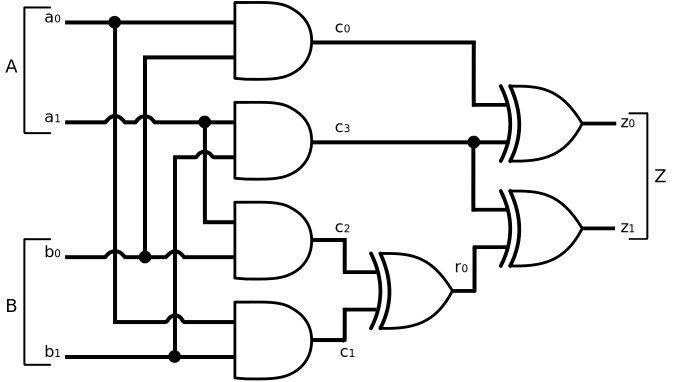
\includegraphics[scale=0.5]{./figures/2bitmasmult.eps}
}
\caption{ A 2-bit multiplier over ${\mathbb{F}}_{2^2}$.}
\label{fig:2bitmul}
\end{figure}

Polynomials extracted from the circuit implementation represent the
ideal $J$. Along with the ideal of vanishing polynomials $J_0$, 
the following polynomials represent the generators 
of $J+J_0$ for the multiplier circuit. 

\begin{eqnarray}
 \left .  
	\begin{aligned}
		f_1:c_0+a_0 \cdot b_0  \\
		f_2:c_1+a_0 \cdot b_1  \\
		f_3:c_2+a_1 \cdot b_0  \\
		f_4:c_3+a_1 \cdot b_1  \\
		f_5:r_0+c_1 + c_2		\\
		f_6:z_0+c_0 + c_3		\\
		f_7:z_1+r_0 + c_3		
	\end{aligned} 
 \ \right\}
 &\qquad&  {\it  \text{Bit-level circuit constraints} ~(\subset J)} \nonumber \\
 \left . 
	\begin{aligned}
		f_{A}:A+a_0+a_1\cdot \alpha   \\ 
		f_{B}:B+b_0+b_1\cdot \alpha  \\ 
		f_{Z}:Z+z_0+z_1\cdot \alpha   
	\end{aligned} 
 \right\}
 &\qquad&  {\it  \text{Word-level designation} ~(\subset J)} \nonumber \\
  \left . 
	\begin{aligned}
		a_0^2-a_0, ~a_1^2-a_1,~b_0^2-b_0, ~b_1^2-b_1   \\ 
		c_0^2-c_0, ~c_1^2-c_1,~c_2^2-c_2, ~c_3^2-c_3  \\ 
		r_0^2-r_0, ~z_0^2-z_0,~z_1^2-z_1    \\ 
		A^4-A, ~B^4-B ,~Z^4-Z		  
	\end{aligned} 
 \right\}
 &\qquad&  {\it \text{vanishing polynomials} (J_0)} \nonumber
\end{eqnarray}
We apply abstraction term order $>$, i.e a lex order with
"bit-level variables" $>$ "Output Z" $>$ "Inputs A, B".

When we compute the reduced \Grobner basis, $G_r$, of \{$J + J_0$\} with 
respect to this ordering, $G_r$ = \{$g_1, \dots, g_{14}\}:$
\begin{align*}
g_1: B^4+B; 
~~g_2: b_0+b_1 \alpha + B; 
~~g_3: a_0+a_1 \alpha + A;  \nonumber \\
~~g_4: c_0+c_1 \alpha + c_2 \alpha + c_3(\alpha+1)+Z;
g_5: r_0+c_1+c_2; 
~~g_6: z_0+c_0+c_3; \nonumber \\
~~g_7: z_1+r_0+c_3; 
~~{\bf g_8: Z+A\cdot B};
~~g_9: b_1+B^2+B; 
~~g_{10}: a_1+A^2+A; \nonumber \\
~~g_{11}: c_3+a_1\cdot b_1
g_{12}: c_2+a_1\cdot b_1 \alpha + a_1 \cdot B; 
~~g_{13}: c_1+a_1\cdot b_1 \alpha +b_1 A; 
~~g_{14}: A^4+A  \nonumber
\end{align*}

$g_8=Z+A\cdot B$ is the {\bf canonical, word-level polynomial } 
representing the function performed by the multiplier $Z=A\cdot B$.
\end{Example}

\section{Conclusion Remarks}
Our approach to word-level abstraction of Galois field arithmetic 
circuits applies concepts of polynomial ideals, varieties, \Grobner basis, 
and abstraction theory to implement verifications on sequential circuits. 
These approaches are described in the following chapters. However, a \Grobner
basis computation is prohibitively expensive; thus we propose improvements 
to our original approach in a subsequent chapter.